\documentclass[10pt]{article}
\author{Alex Peyrard}
\title{Digital Image Processing}
\usepackage{graphicx}

\begin{document}
\maketitle
\section{Introduction}
All of the programs are written in python 3. The shebangs are included and thus they should work if called using the "./program.py" notation. In case this causes a problem, please try to call them using "python3 program.py" notation.\\\\
I will provide further help on how to call each program.
\subsection{libraries}
I used numpy in all of the programs and scipy in some of them. I will detail when scipy is used.
\section{Exercise 1}
The program called ex1.py computes the histogram of a greyscale image, and enhances the image using histogram equalization. it displays the enhanced image, the histograms of the default and enhanced images, and the transformation function.
\subsection{Examples}
\subsubsection{Fig1.jpg}
All of the results are obtained using the program with the call "./ex1.py Fig1.jpg"
\begin{figure}[!ht]
	\centering
	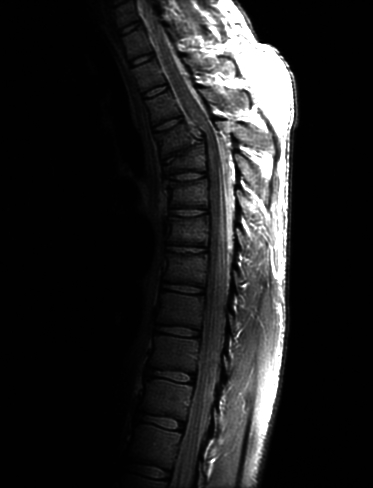
\includegraphics[height=200pt]{./ex1/Fig1.jpg}
	\caption{Original image}
\end{figure}
\begin{figure}[!ht]
	\centering
	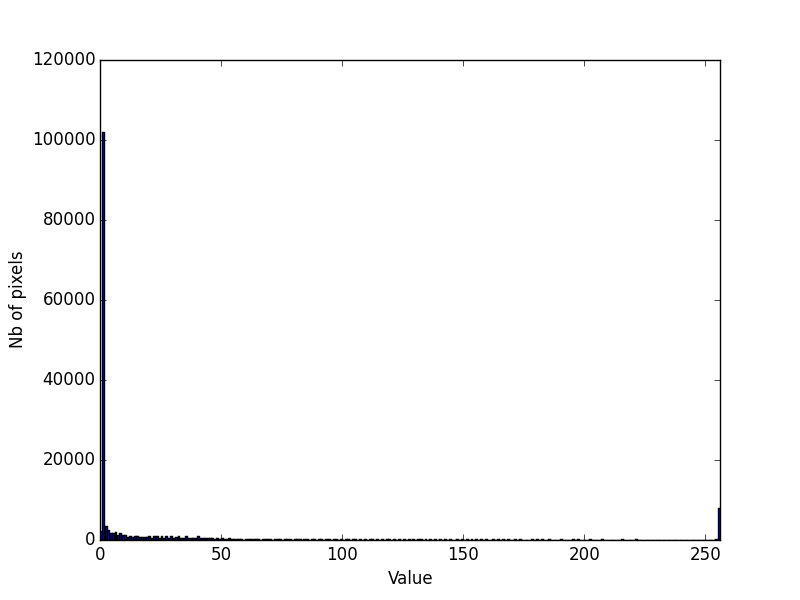
\includegraphics[height=200pt]{./ex1/Fig1_hist.png}
	\caption{Original image's histogram}
\end{figure}
\begin{figure}[!ht]
	\centering
	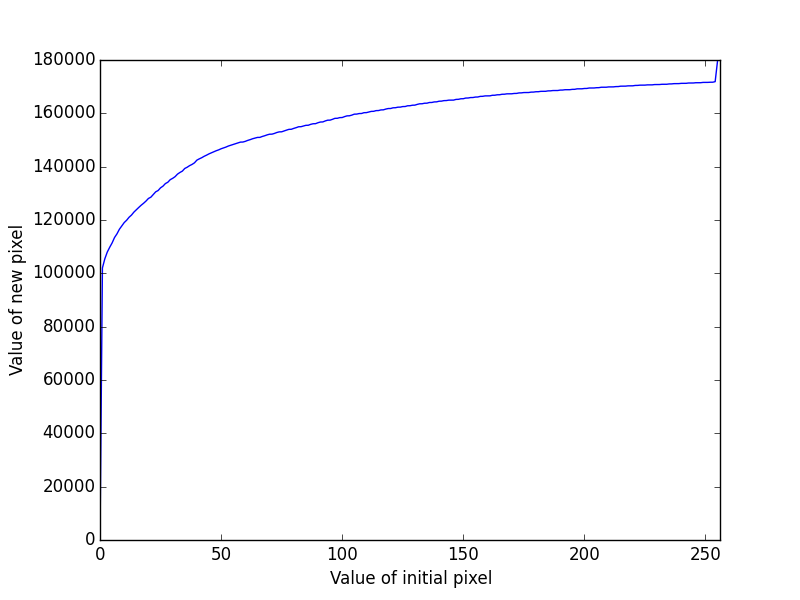
\includegraphics[height=200pt]{./ex1/Fig1_cdf.png}
	\caption{Enhancement function}
\end{figure}
\begin{figure}[!ht]
	\centering
	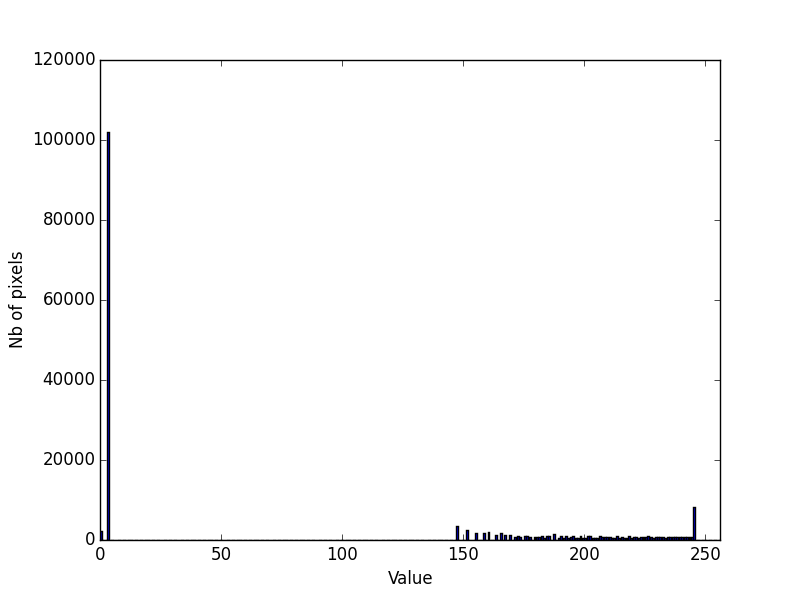
\includegraphics[height=200pt]{./ex1/Fig1_enh_hist.png}
	\caption{Enhanced image histogram}
\end{figure}
\begin{figure}[!ht]
	\centering
	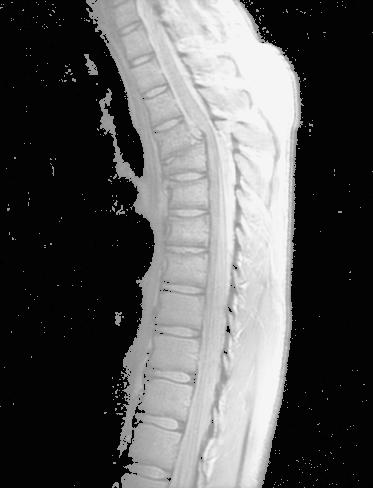
\includegraphics[height=200pt]{./ex1/Fig1_enh.jpg}
	\caption{Enhanced image}
\end{figure}
\clearpage

\subsubsection{Fig2.jpg}
All of the results are obtained using the program with the call "./ex1.py Fig2.jpg"
\begin{figure}[!ht]
	\centering
	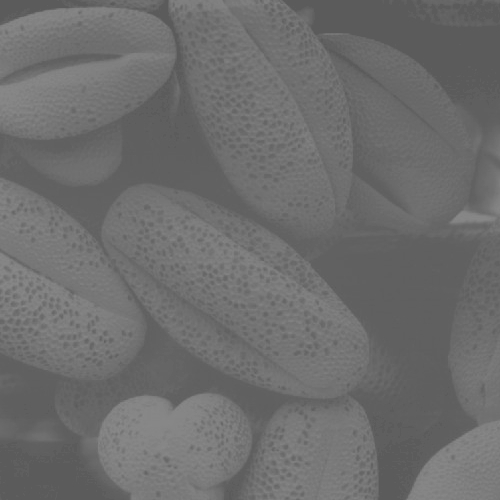
\includegraphics[height=200pt]{./ex1/Fig2.jpg}
	\caption{Original image}
\end{figure}
\begin{figure}[!ht]
	\centering
	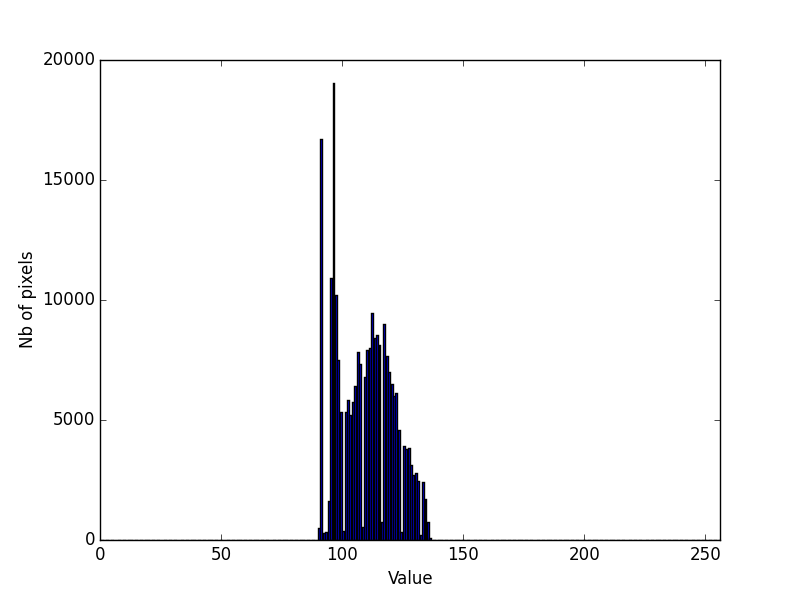
\includegraphics[height=200pt]{./ex1/Fig2_hist.png}
	\caption{Original image's histogram}
\end{figure}
\begin{figure}[!ht]
	\centering
	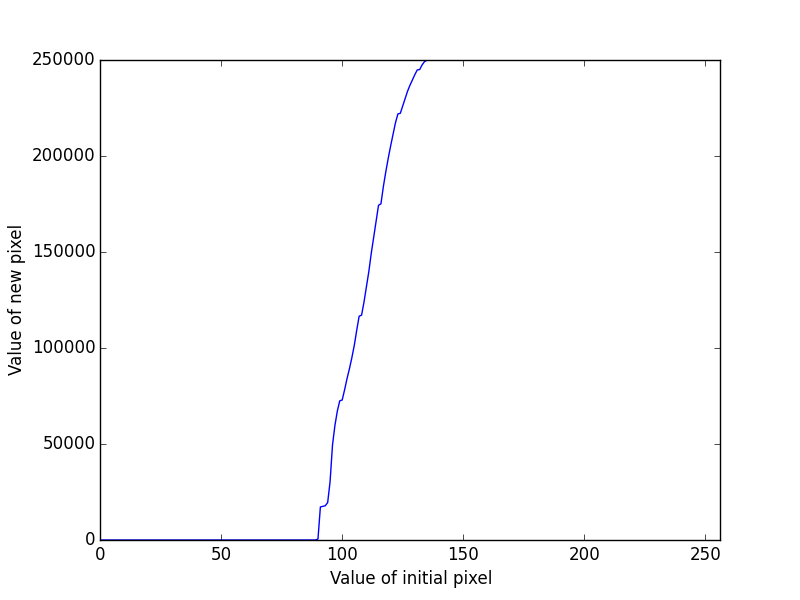
\includegraphics[height=200pt]{./ex1/Fig2_cdf.png}
	\caption{Enhancement function}
\end{figure}
\begin{figure}[!ht]
	\centering
	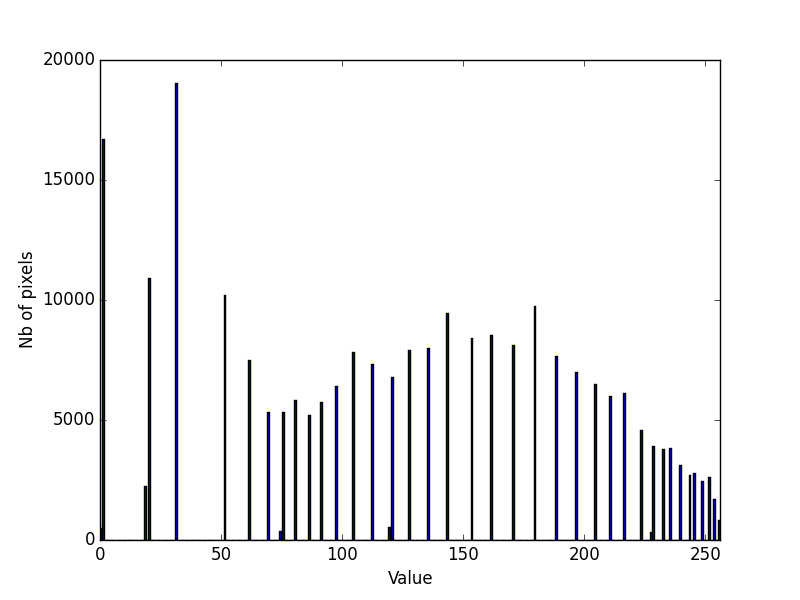
\includegraphics[height=200pt]{./ex1/Fig2_enh_hist.png}
	\caption{Enhanced image histogram}
\end{figure}
\begin{figure}[!ht]
	\centering
	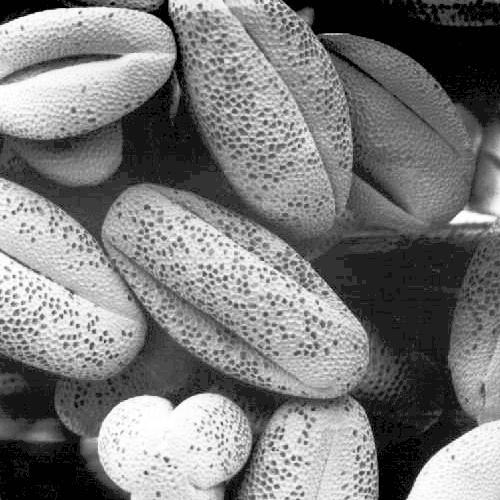
\includegraphics[height=200pt]{./ex1/Fig2_enh.jpg}
	\caption{Enhanced image}
\end{figure}
\clearpage

\section{Exercise 2}

\end{document}